\section{Übersicht}

Bevor ich auf meine Forschung im Detail eingehe, stelle ich in diesem Abschnitt zunächst vor, in welchem Kontext meine Arbeit eingebettet war. Aus diesem Kontext heraus hat sich eine etwas native Planung für das Forschungsvorhaben ergeben. Diese Planung stelle ich in diesem Abschnitt genauso vor, wie deren Abweichungen. Abschließend gehe ich auf Schwierigkeiten meiner Forschung ein, die u.a. die Abweichungen zur ursprünglichen Planung erklären.


\subsection{Rahmenbedingungen}
\label{sec:rahmenbedingungen}
Diese Dissertation entstand im Rahmen meiner Tätigkeit im \textit{BioStore}-Projekt.

Das in der Arbeitsgruppe \textit{Algorithmische Bioinformatik}\footnote{\url{https://www.mi.fu-berlin.de/en/inf/groups/abi/index.html}} von Prof. Dr. Knut Reinert angesiedelte BioStore-Projekt wurde durch das \textit{Bundesministerium für Bildung und Forschung} (\textit{BMBF})\footnote{\url{http://www.bmbf.de}} im Rahmen des Programms \textit{VIP --- Validierung des Innovationspotenzials wissenschaftlicher Forschung}\footnote{\url{http://www.validierungsfoerderung.de/mediathek/vip-projektfilm-biostore}} für einen Zeitraum von drei Jahren bis einschließlich Juli 2014 gefördert.

\begin{figure}[ht!]
  \centering
    
\includegraphics[width=0.3\linewidth]{Figures/biostore-logo.png}
  \caption[BioStore-Logo]{Logo des BioStore-Projekts}
  \label{fig:biostore-logo}
\end{figure}

Das BioStore-Projekt hatte das Ziel zu untersuchen, ``wie Computerprogramme zur Anwendung einer neuen Generation von Genomsequenz-Daten effizient entwickelt und vertrieben werden können'' \citep{Reinert:tg} und dies mittels eines App-Stores für bioinformatische standardisierte Werkzeuge --- ``BioStore'' genannt --- zu demonstrieren. Ein ebenfalls bereitgestelltes Workflow-Modul sollte, ähnlich zu Endanwender-Entwicklungsumgebungen, dem Anwender erlauben, bioinformatische Komponenten aus dem BioStore zu beziehen und zu Workflows zu komponieren. \citep{Reinert:tg,Reinert:2011vl}

\begin{figure}
  \centering
    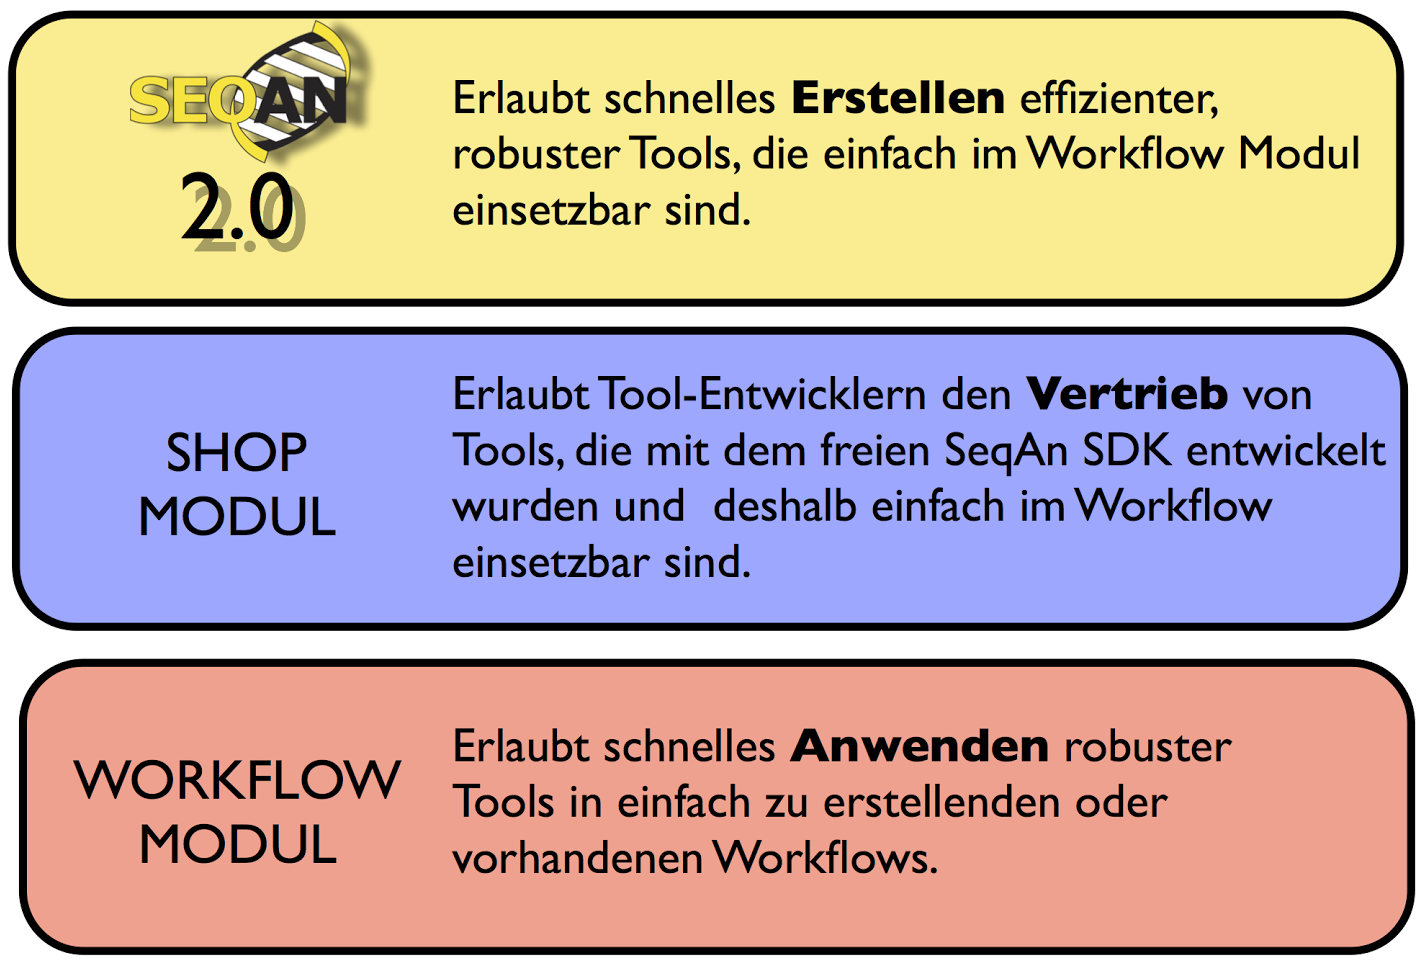
\includegraphics[width=0.6\linewidth]{Figures/seqan20.png}
  \caption[BioStore-Komponenten]{Komponenten des BioStore-Projekts \citep{Reinert:2011vl}}
  \label{fig:biostore-demonstrator}
\end{figure}

Ich besetzte innerhalb dieses Projekts die Stelle des Usability-Spezialisten, der für die Usability-Verbesserung der Softwarebibliothek SeqAn zuständig war. SeqAn spielte im Rahmen von BioStore eine primäre Rolle, da praktisch alle bereitgestellten Bioinformatik-Werkzeuge auf SeqAn basierten (siehe \sref{sec:seqan-tools}). Der zweite Schwerpunkt meiner Projekttätigkeit bestand in der Mitarbeit am BioStore selbst und am Workflow-Modul. Aus ökonomischen Gründen musste der Umfang des Projekts auf Seiten der Arbeitsgruppe gekürzt werden. Anstelle eines eigenen Shops und eines eigenen Workflow-Moduls wurde die Workflow-Engine \textit{KNIME Analytics Platform}\footnote{\url{http://www.knime.org/knime}} (kurz: KNIME) verwendet und erweitert. Die Arbeiten an KNIME fielen somit unter anderem in meinen Zuständigkeitsbereich.



\subsection{Planung}

\label{sec:data-sources-workshop}
Im Rahmen des dreijährigen BioStore-Projekts sollten drei Workshops stattfinden, die sich an Interessierte aus der Bioinformatik und verwandten Wissenschaften richteten\footnote{\url{http://www.seqan-biostore.de/wp/seqan-workshops/}}. Ziel der Workshops war es, den Anwendern SeqAn theoretisch wie auch praktisch vorzustellen und den Teilnehmern die Möglichkeit zu geben, ihre auf SeqAn-basierten Projekte vorzustellen. Für den praktischen Teil wurden vornehmlich die online-verfügbaren SeqAn-Tutorials\footnote{\url{http://seqan.readthedocs.org/en/master/Tutorial.html}} gemeinsam mit den Workshop-Teilnehmer interaktiv bearbeitet. Ein solcher Workshop bot also die ideale Möglichkeit, Forschungsdaten zur Analyse und Verbesserung der API-Usability von SeqAn im Rahmen einer explorativen empirischen Fallstudie zu erheben.

Die ursprüngliche Planung bestand aus den folgenden Phasen:

\begin{description}
  \item[1.Datenerhebung] \hfill \\
  Es war vorgesehen, objektive Daten zu erheben. Diese Daten sollten die Entwicklungsschritte der von den SeqAn-Workshop-Teilnehmern entwickelten Programme dokumentieren. Diese Datenquelle wird im Folgenden als \textit{Programmierfortschritte}-Datenquelle bezeichnet und im \sref{sec:programmierfortschritte} genauer vorgestellt.
  \item[2. Datenanalyse] \hfill \\
  Die erhobenen Daten sollten mit Hilfe der \gls{gtm} analysiert werden. Dieser Schritt sollte die vorhandenen API-Usability-Probleme nicht nur aufdecken, sondern auch ein grundlegendes Verständnis verschaffen.
  \item[3. API-Usability-Verbesserung] \hfill \\
  Auf der Grundlage der Analyseergebnisse sollten Verbesserungsvorschläge für die API von SeqAn formuliert und umgesetzt werden.
  \item[4. Validierung] \hfill \\
  Mit einer weiteren Datenerhebung und -analyse mittels \gls{gtm} sollte die Effektivität der zuvor umgesetzten Usability-Verbesserungen validiert werden. Die Verbesserungen mussten also spätestens bis zum dritten und letzten Workshop umgesetzt worden sein, um eben diesen Workshop als letzte Möglichkeit der Datenerhebung für die Validierung nutzen zu können.
\end{description}



\subsection{Tatsächlicher Verlauf}
\label{sec:verlauf}

Der zeitliche Verlauf wich stark von der ursprünglichen Planung ab. Dies ist im Grunde nicht weiter erstaunlich, ist die von mir verwendete \gls{gtm} doch ein sehr offener --- weil explorativer --- Forschungsansatz.

\label{sec:data-sources-pmsb}
Neben den SeqAn-Workshops bot sich eine weitere Datenquelle an, nämlich das jährlich stattfindende Bioinformatik-Praktikum \textit{Projektmanagement im Softwarebereich (PMSB)}\footnote{\url{http://www.mi.fu-berlin.de/w/ABI/LectureWiki}} des Fachbereichs Mathematik und Informatik der Freien Universität Berlin. Innerhalb dieses Praktikums erhalten die teilnehmenden Studenten eine 4-tägige Einführung in SeqAn, bei der die von den Workshops bekannten Tutorials eingesetzt werden. Der Einführung schließt sich eine einmonatige Projektarbeit an, bei der SeqAn zum Einsatz kommt. Drei dieser Veranstaltungen lagen in dem ursprünglich geplanten Zeitraum für diese Arbeit und boten sich so ebenfalls für die Datenerhebung an.

\bigskip

Die vier größten Schwierigkeiten bei der Einhaltung der ursprünglichen Planung waren:
\begin{description}
  \item[Organisatorische Restriktionen] Abgesehen von möglichen Langzeitbeobachtungen\footnote{Diese Datenquelle war die einzige, bei der ich hohe organisatorische Freiheitsgrad bzgl. der Durchführung hatte. Darauf gehe ich genauer im \sref{sec:phase2-programmierfortschritte-durchfuhrung} auf Seite \pageref{sec:phase2-programmierfortschritte-durchfuhrung} ein.} gab es nur die SeqAn-Workshops und die hinzugekommenen PMSB-Praktika, deren zeitliche Planung sich an anderen Faktoren orientierte als meiner Forschung. Dieser Umstand führte dazu, dass jede Möglichkeit zur Datenerhebung genutzt und so umfassend wie möglich sein musste. Schließlich erfordert die korrekte Anwendung der \gls{gtm} für die Klärung von Theorielücken weitere Datenerhebungen (\textit{theoretisches Sampling}) durchzuführen.
  \item[Unübliches Datenformat] Die Art der erhobenen Daten machte die Entwicklung eines Werkzeugs zur Datenvisualisierung notwendig. Jedoch erforderte der Einsatz der \gls{gtm} eine entsprechende technische Unterstützung. Diese Erkenntnis machte den Ausbau des Datenvisualisierungswerkzeugs zu einem qualitativen Datenanalysewerkzeug notwendig, dessen Entwicklung weit mehr Zeit in Anspruch nahm, als ich annahm. Dieses Werkzeug mit dem Namen \acrlong{apiua} stelle ich im \sref{sec:apiua} vor.
  \item[Unreife Usability] Bereits bei der Vorbereitung und Durchführung der ersten Datenerhebung und spätestens bei der Analyse dieser Daten wurde klar, dass SeqAn unter teils offensichtlichen und in der Literatur längst bekannten API-Usability-Problemen litt. Diese Probleme dominierten die Daten so stark, dass die interessanteren und fundamentaleren Probleme kaum noch zu beobachten waren oder gar nicht erst auftraten. Darum mussten die groben API-Usability-Probleme zunächst zeitraubend beseitigt werden.
\end{description}

\bigskip

Retrospektiv betrachtet ergab sich der folgende, vereinfacht dargestellte Verlauf (vgl. \fref{fig:forschung-ablauf}):

\begin{enumerate}
  \item Erste Datenerhebung (Workshop'11)\footnote{Ich verwende die Notation \textit{'xx} für die Darstellung des Jahres, in dem eine Veranstaltung stattfand. \textit{`11} steht beispielsweise für das Jahr \textit{2011}.}
  \item Implementierung eines Werkzeugs zur Datenvisualisierung / -exploration 
  \item Zweite Datenerhebung (PMSB'12)
  \item Datenanalyse (Workshop'11 und PMSB'12)\\und parallele Weiterentwicklung des Datenvisualisierungswerkzeugs zu einem Datenanalysewerkzeug, das später den Namen \textit{\gls{apiua}} erhielt
  \item Behebung grober API-Usability-Probleme
  \item Dritte Datenerhebung (Workshop'12)
  \item Literaturforschung
  \item Datenanalyse (Workshop'11 und PMSB'12)\\und bedarfsgetriebene parallele Weiterentwicklung von \gls{apiua}
  \item Vierte Datenerhebung (PMSB'13)
  \item Abschluss der Behebung grober API-Usability-Probleme\\(insbesondere Dokumentation)
  \item Fünfte Datenerhebung (Workshop'13)
  \item Datenanalyse (Workshop'13-Fragebögen)\\und bedarfsgetriebene parallele Weiterentwicklung von \gls{apiua}
  \item Datenanalyse (Workshop'12-Gruppendiskussion)
  \item Verifikation der Erkenntnisse an Hand der Datenquelle \textit{Programmierfortschritte}
  \item Synthese der Forschungsergebnisse
  \item Formulierung von API-Usability-Verbesserungsvorschlägen
\end{enumerate}

\newgeometry{inner=2cm,outer=1.5cm,top=1.5cm,bottom=1.5cm}
\thispagestyle{empty}
\begin{landscape}
\begin{figure}
  \centering
    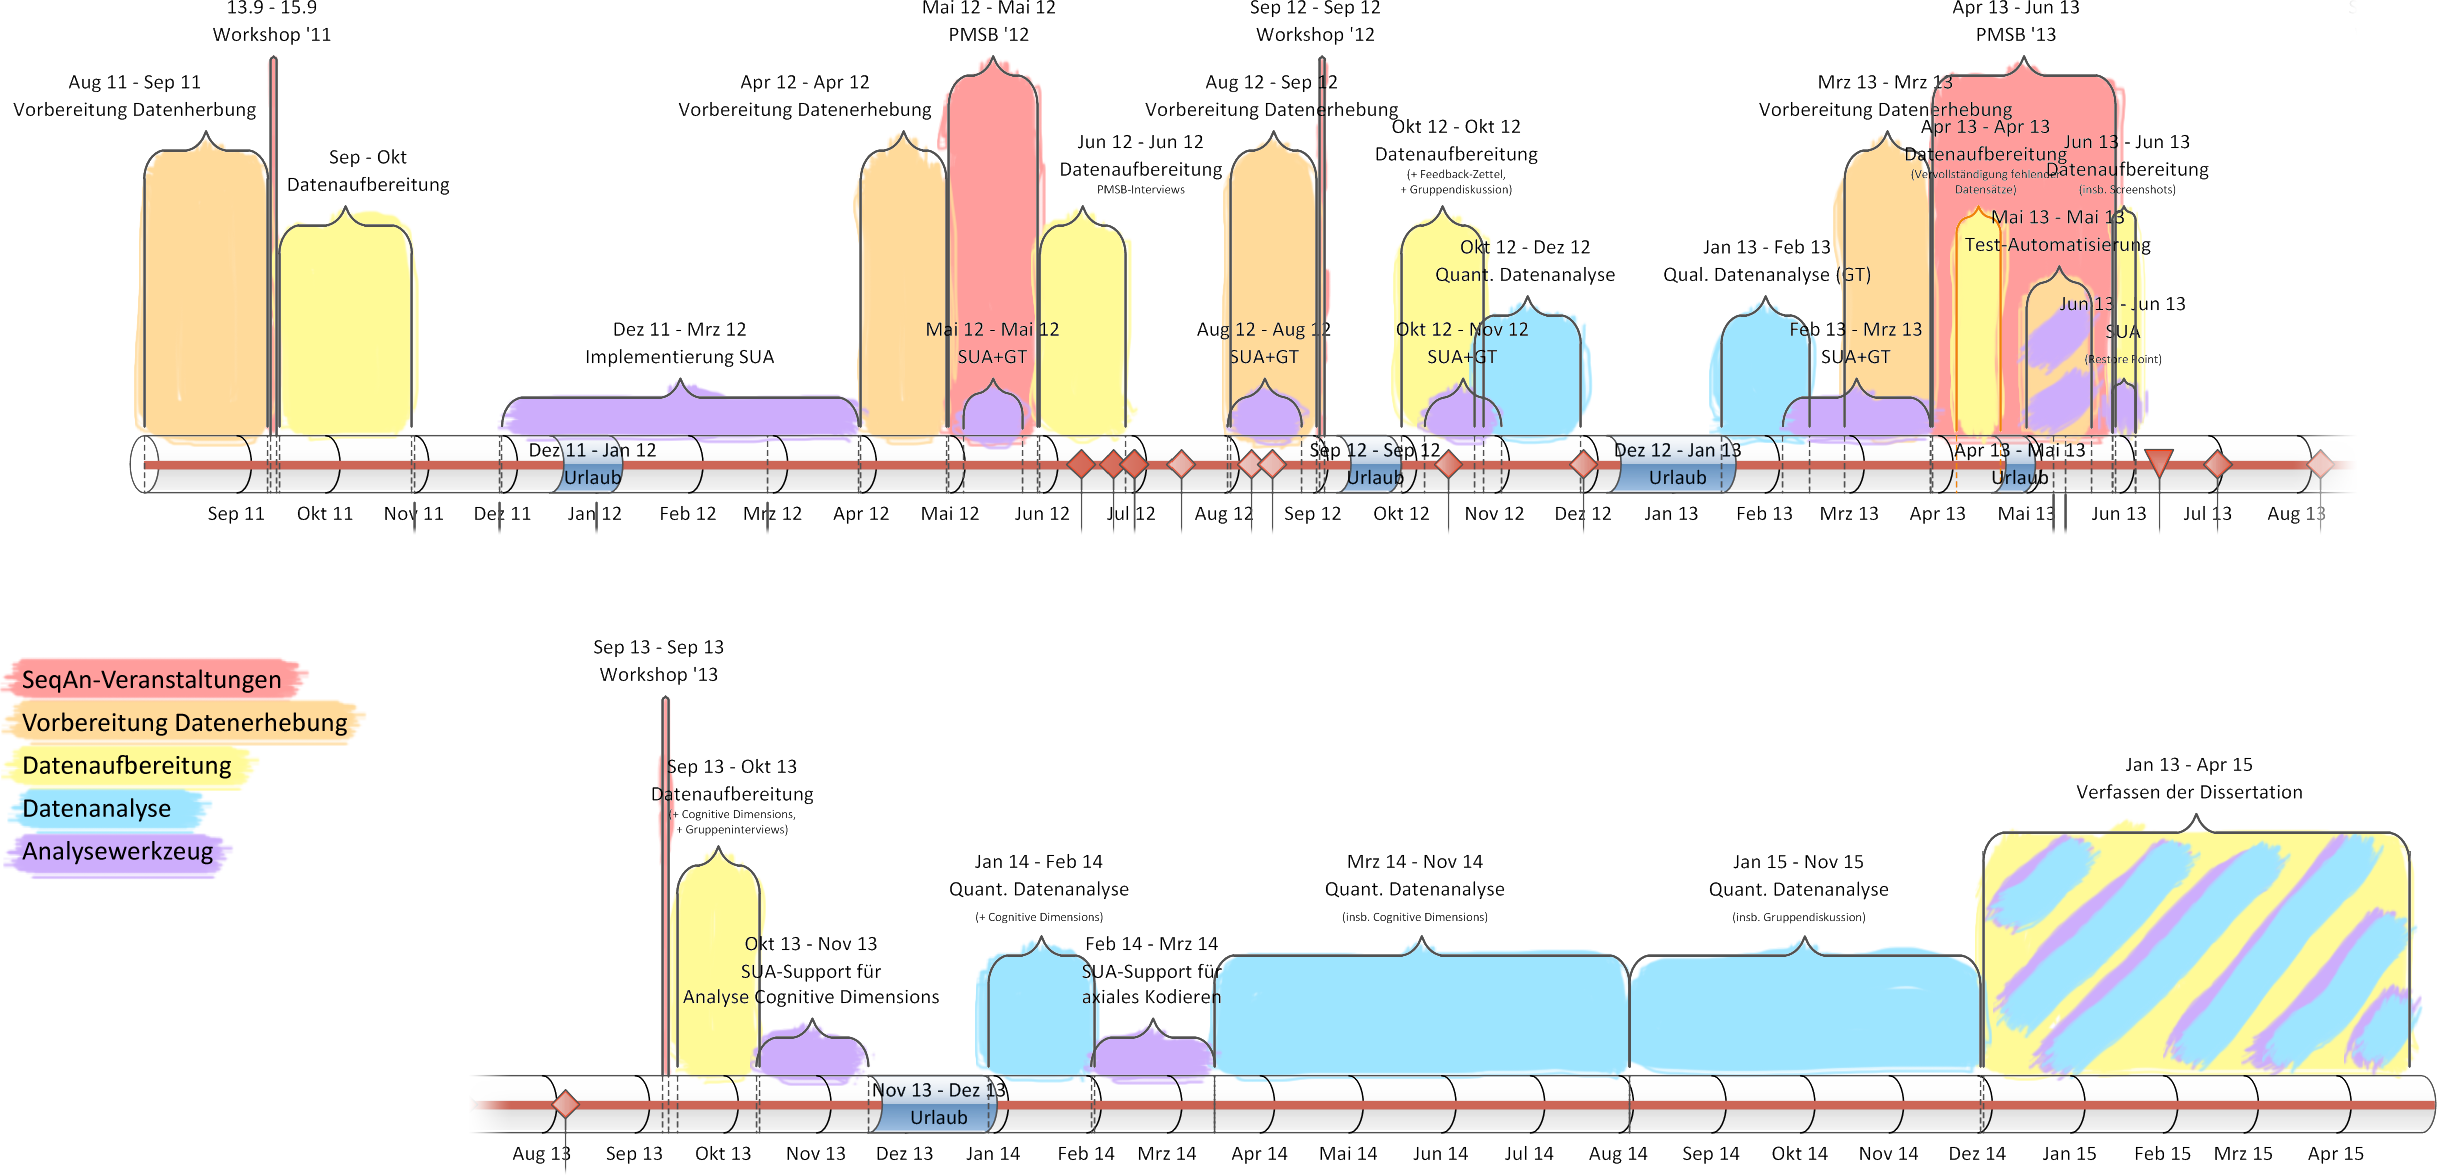
\includegraphics[width=1.0\linewidth]{Figures/forschung-ablauf.png}
  \caption[Zeitlicher Verlauf dieser Arbeit]{Zeitlicher Verlauf dieser Arbeit\\Datenerhebungen sind rot, Datenerhebungsvorbereitungen orange, Datenerhebungsnachbereitungen gelb, Datenanalysen blau und Arbeiten am Datenanalysewerkzeug violett dargestellt.}
  \label{fig:forschung-ablauf}
\end{figure}
\end{landscape}
\restoregeometry

Die zwei wichtigsten Auffälligkeiten sind einerseits die zusätzlichen Datenerhebungen während zwei PMSB-Praktika und andererseits der große Zeitbedarf der \gls{apiua}-Entwicklung.

Im Verlauf meiner Forschung stellte sich schnell heraus, dass meine Unerfahrenheit im Umgang mit der \gls{gtm}, gepaart mit der speziellen Gestalt der erhobenen Programmierfortschritte-Daten zu zeitintensiv sein würde, um das Ziel der Verbesserung der API von SeqAn zu erreichen. Ich musste zunächst Erfahrungen im Gebrauch der \gls{gtm} sammeln und meine \textit{theoretische Sensibilität} schärfen. Aus diesen Gründen entschloss ich mich, zunächst subjektive Datenquellen wie Fragebögen, Interviews und Gruppendiskussionen für die Datenerhebung zu verwenden und zu analysieren. Dieser Methodenmix hatte den Vorteil, dass ich so auch APU-Usability-Probleme aufdecken konnte, die nur in einer der Datenquellen zu finden waren. Außerdem wurde dieses Vorgehen dem Gütekriterium \textit{Triangulierung} \citep{mayring2002einfhrung} gerechter.

Aus diversen, im \href{sec:schwierigkeiten}{nächsten Abschnitt beschriebenen Schwierigkeiten} musste ich von der Planung Abstand nehmen, eine empirische Validierung der API-Usability-Verbesserungen vorzunehmen.



\subsection{Schwierigkeiten}
\label{sec:schwierigkeiten}

\subsubsection{Wissenschaftliche und methodische Schwierigkeiten}

Die Einarbeitung in das Gebiet der API-Usability war unerwartet aufwändig, da es keine umfassenden, über ``den Tellerrand'' schauenden, wissenschaftlichen Literaturstudien gab. Eine solche Literaturstudie musste ich also zunächst erarbeiten.

Diese im vorangegangen Kapitel vorgestellte \href{sec:forschungsstand}{Literaturstudie} --- insbesondere \cite{Robillard:2010bh,Eisenberg:2010bm,Stylos:2009bq,Stylos:2008jt,Ellis:2007kv} --- zeigt, dass sich die Forschung häufig nur auf kleine definierte API-Usability-Aspekte konzentrierte. Entsprechend sinnvoll war die Verwendung der sich für explorative Studien besonders geeigneten \gls{gtm}.
\\Die Verwendung der \gls{gtm} ist für einen Informatiker jedoch nicht einfach und selbst empirische Forschung findet in der Informatik wenig statt. In einer Literaturstudie von 1995-1999 fanden \cite{Glass:2002ec} heraus, dass nur ein Bruchteil der veröffentlichten Studien empirisch zu Stande gekommen ist und gerade einmal 2\% der Arbeiten Bezug auf andere Disziplinen genommen haben. Außerdem habe ich im \sref{sec:gtm-informatik} dargestellt, wie wenig Studien überhaupt die \gls{gtm} einsetzen. Unter den mit bekannten \gls{gtm}-Studien befindet sich nicht eine, die tatsächlich eine \gls{gt} vorgestellt hat. Bei der Hälfte wurde die \gls{gtm} nur in unzureichender Weise angewandt.
\\Für die Erforschung der API-Usability-Forschung mittels \gls{gtm} gibt es keine Studie, an der ich mich methodisch orientieren konnte. Entsprechend eigenständig musste ich also die Datenerhebung und -analyse individuell planen und realisieren.

Forscher, die ein gutes Verständnis von API-Usability und von ihrem fachlichen Forschungsgegenstand haben, sind rar \citep{DaqingHou:2005ba}. Dies trifft auch auf Informatik und Bioinformatik zu \citep{Tisdall:2001td}. In Bezug auf Bioinformatiker als Anwendergruppe gibt es kaum Forschung \citep{Letondal:2006dy}. Das spezielle Datenerhebungsverfahren und der ihm geschuldete Bau eines Datenanalysewerkzeugs gestaltete das Vorhaben nicht einfacher.

%Kurzum: Als Informatiker die vergleichsweise schlecht erforschte API-Usability einer auf Templatemetaprogrammierung-basierenden Bioinformatik-Softwarebibliothek mittels \gls{gtm} zu verbessern, ist kein triviales Unterfangen. 

Die oben genannten Gründe und Zeitprobleme zwangen mich zu einer kostengünstigen Validierung meiner Arbeit. Diese scheiterte jedoch an der, nicht ohne weiteres ersichtlichen Unreife des Cognitive Dimension Frameworks (siehe \sref{sec:cdf-validation-difficulties}), welches ich für diesen Zweck verwenden wollte. Darum musste ich mich gegen eine empirische und für eine argumentative Validierung entschließen. 

Auf Seiten der Bioinformatik-Arbeitsgruppe gab es andere Vorstellungen von meiner Arbeit im BioStore-Projekt. Mein Promotionsziel und den API-Usability-Forschungsstand übersehend, wurden quantitative, zeitnahe und unmittelbar umsetzbare Forschungsergebnisse erwartet. Ich führe dies auf den quantitativen Forschungsschwerpunkt der Bioinformatik, einer gewissen Unerfahrenheit mit qualitativer Forschung\footnote{Äußerungen der Mitglieder der Bioinformatik-Arbeitsgruppe in persönlichen Gesprächen, wie auch bei der Präsentation von Zwischenergebnissen gaben Aufschluss über die existierende Skepsis gegenüber und Unerfahrenheit mit qualitativer Forschung.} und auf die zeitliche Begrenzung des BioStore-Projekts zurück.



\subsubsection{Organisatorische Schwierigkeiten}

\paragraph{Aufgaben}

Häufig sind Forscher, die ein Promotionsziel verfolgen, mit der Tatsache konfrontiert, dass auch andere Aufgaben in ihren Arbeitsbereich fallen. In meinem Fall gehörten zu diesen Aufgaben die Arbeit an der Workflow-Engine KNIME, die im ersten Jahr mehrere Monate umfasste.

Die geforderten quantitativ-konstruktiven Forschungsergebnisse belasteten mich jedoch mehr, denn sie waren nicht nur zeitraubend und für meine Promotion von nur geringer Relevanz, sondern dienten auch dem Projekt nur als kosmetischer Balsam für die Entwickler-Ehre und weniger zur grundlegenden Usability-Verbesserung der SeqAn-API.
\\Ich habe die These, dass Teile der SeqAn-Entwickler von der Usability der Softwarebibliothek bereits überzeugt waren. Starke Indizien dafür sind \textit{Bauchgefühl-Usability}\footnote{Damit bezeichne ich die \textit{intuitive} (im Gegensatz zur \textit{argumentativen} oder \textit{empirischen}) Entscheidungsfindung in Bezug auf Usability-relevante Entwurfsentscheidungen. Im \sref{sec:bauch-usability} beschreibe ich dieses Konzept ausführlicher.}
und \textit{technisches Wegargumentieren}\footnote{Dieses Konzept wird von \cite{Sarodnick:2006vc} anekdotisch beschrieben. Dabei tendieren Softwareentwickler stark dazu, Eindrücken ihrer Anwenderschaft --- berechtigt oder nicht --- mit technischen Argumenten zu begegnen. Diese Erfahrung machte ich selbst bereits bei der ersten Feedback-Runde während des ersten SeqAn-Workshops. Im \sref{sec:gruppendiskussion} bespreche ich die daraus gezogenen Konsequenzen für meine Datenerhebung.}.

Es boten sich sechs Datenerhebungsmöglichkeiten (drei SeqAn-Workshops, drei PMSB-Praktika). Eine einzelne Datenerhebung forderte einen erheblichen Vor- und Nachbereitungsaufwand. Noch weitaus schwerer wog der Aufwand für die Analyse eines solchen Datensatzes. Auch wenn es illusorisch war, alle Datensätze zu analysieren, erntete ich mit meiner Entscheidung, die letzte Datenerhebungsmöglichkeit aus zeitlichen und inhaltlichen Gründen nicht mehr zu nutzen, größtenteils Unverständnis.

Meine Stellung in der Bioinformatik-Arbeitsgruppe (AGABI) war durch meine wissenschaftliche Zugehörigkeit zur Arbeitsgruppe \textit{Software Engineering} (AGSE) diffus, was sich selbst in einer Diskussion zu den Schließrechten der entsprechenden Räumlichkeiten zeigte. Dies führte in Verbindung mit meiner, eben geschilderten Unzufriedenheit zu einer unbewussten Entfernung von der AGABI, was aber auch in einen geringeren Informationsfluss mündete. 

\paragraph{Projekt}

Auf Projekt-Ebene gestaltete sich die Erarbeitung dieser Dissertation schwierig, denn das BioStore-Projekt war auf drei Jahre beschränkt --- und damit auch die Bezahlung des Personals. Dies führte zu finanziellen Problemen meinerseits. Meine Erfahrung mit anderen Kollegen zeigte mir, dass der erfolgreiche Abschluss der Promotion nur in Vollzeit möglich ist. Diese Monate musste ich mir mit meinen knappen Ersparnissen finanzieren und mich finanziell auf das Nötigste reduzieren.

Die inhaltliche Arbeit erschwerte sich durch den Projektende-bedingten Wegfall wichtiger Projektmitglieder, zu denen insbesondere zwei SeqAn-Hauptentwickler gehörten. Dadurch rutschte die Umsetzung wichtiger API-Usability-Verbesserungen in weite Ferne --- beziehungsweise in den \href{sec:ausblick}{Ausblick dieser Arbeit}. Diese Entwicklung machte die empirische Validierung dieser Verbesserungsvorschläge unmöglich.

\paragraph{Technik}

Die personelle Dynamik setzte sich in der eigentlichen SeqAn-Softwarebibliothek fort, denn sie wurde natürlich während meiner Arbeit stetig im Sinne des BioStore-Projekts funktionell (z.B. IO-Modul, Parallelisierung) und strukturell (z.B. Beseitigung von Forward-Declarations) weiterentwickelt. Zu diesen Änderungen gehörten allerdings auch eigenmächtige Bauchgefühl-Usability-Verbesserungen wie dem Wechsel der Tutorial-Dokumentationsplattform von \textit{trac}\footnote{\url{http://trac.edgewall.org}}, hin zur auf \textit{Sphinx}\footnote{\url{http://sphinx-doc.org}}-basierenden \textit{Read the Docs}-Plattform\footnote{\url{http://seqan.readthedocs.org}}.

%- Bibliotheksumstrukturierungen (Beseitigung von forward declarations, Parallelisierung (mit GPU), Herausarbeitung von Apps in eigene Github-Repositories)

Darüber hinaus hat sich sogar die, SeqAn zu Grunde liegende Programmiersprache C{}\verb!++! weiterentwickelt. Anpassungen an den C{}\verb!++!11-Sprachstandard wurden in SeqAn Mitte 2014 angefangen und mittlerweile zum Abschluss gebracht.

\bigskip

Im Folgenden werde ich eine --- von den oben genannten Schwierigkeiten weitestgehend bereinigte --- Darstellung meiner Forschung vornehmen und sie nicht rein zeitlich, sondern vornehmlich inhaltlich gliedern. Um den Lesefluss und das Verständnis dieser Arbeit nicht unnötig zu erschweren, nehme ich nur an Stellen Bezug auf diese Schwierigkeiten, wenn es der Nachvollziehbarkeit dienlich ist.